%%%%%%%%%%%%%%%%%%%%%%%%%%%%%%%%%%%%%%%%%%%%%%%%%%%%%%%%%%%%%%%%%%%%%%%%%%%%%%%
% Sign Language Detection using Faster R-CNN - Project Report
% Author: Ammar Riaz (2023377)
% Course: AI331L - Deep Neural Networks Lab
% Program: BS Artificial Intelligence
%%%%%%%%%%%%%%%%%%%%%%%%%%%%%%%%%%%%%%%%%%%%%%%%%%%%%%%%%%%%%%%%%%%%%%%%%%%%%%%

\documentclass[12pt,a4paper]{article}

% ============== PACKAGES ==============
\usepackage[utf8]{inputenc}
\usepackage[T1]{fontenc}
\usepackage{lmodern}
\usepackage[margin=1in]{geometry}
\usepackage{graphicx}
\usepackage{amsmath,amssymb,amsfonts}
\usepackage{algorithm}
\usepackage{algpseudocode}
\usepackage{listings}
\usepackage{xcolor}
\usepackage{hyperref}
\usepackage{booktabs}
\usepackage{multirow}
\usepackage{caption}
\usepackage{subcaption}
\usepackage{float}
\usepackage{enumitem}
\usepackage{fancyhdr}
\usepackage{tikz}
\usetikzlibrary{shapes,arrows,positioning,fit,backgrounds}
\usepackage{pgfplots}
\pgfplotsset{compat=1.17}
\usepackage{tcolorbox}
\usepackage{array}
\usepackage{longtable}
\usepackage{cite}
\usepackage{url}
\usepackage{setspace}

% ============== CONFIGURATION ==============
\hypersetup{
    colorlinks=true,
    linkcolor=blue,
    filecolor=magenta,
    urlcolor=cyan,
    citecolor=green,
    pdftitle={Sign Language Detection using Faster R-CNN},
    pdfauthor={Ammar Riaz},
}

% Code listing style
\definecolor{codegreen}{rgb}{0,0.6,0}
\definecolor{codegray}{rgb}{0.5,0.5,0.5}
\definecolor{codepurple}{rgb}{0.58,0,0.82}
\definecolor{backcolour}{rgb}{0.95,0.95,0.92}

\lstdefinestyle{mystyle}{
    backgroundcolor=\color{backcolour},
    commentstyle=\color{codegreen},
    keywordstyle=\color{magenta},
    numberstyle=\tiny\color{codegray},
    stringstyle=\color{codepurple},
    basicstyle=\ttfamily\footnotesize,
    breakatwhitespace=false,
    breaklines=true,
    captionpos=b,
    keepspaces=true,
    numbers=left,
    numbersep=5pt,
    showspaces=false,
    showstringspaces=false,
    showtabs=false,
    tabsize=2,
    frame=single
}
\lstset{style=mystyle}

% Header and footer
\pagestyle{fancy}
\fancyhf{}
\rhead{AI331L - DNN Lab}
\lhead{Sign Language Detection}
\cfoot{\thepage}

% ============== DOCUMENT START ==============
\begin{document}

%%%%%%%%%%%%%%%%%%%%%%%%%%%%%%%%%%%%%%%%%%%%%%%%%%%%%%%%%%%%%%%%%%%%%%%%%%%%%%%
% TITLE PAGE
%%%%%%%%%%%%%%%%%%%%%%%%%%%%%%%%%%%%%%%%%%%%%%%%%%%%%%%%%%%%%%%%%%%%%%%%%%%%%%%
\begin{titlepage}
    \centering
    \vspace*{1cm}
    
    % University Logo placeholder
    
\begin{tikzpicture}
        \node[draw, circle, minimum size=3cm, line width=2pt, color=blue!70] (logo) {};
        \node at (logo.center) {\textbf{\Large University}};
    \end{tikzpicture}
    
    \vspace{1.5cm}
    
    {\Huge\bfseries Sign Language Detection Using\\[0.3cm] Faster R-CNN with FastAPI Deployment\par}
    
    \vspace{1cm}
    
    {\Large\itshape Real-time American Sign Language Alphabet Recognition\\using Deep Learning Object Detection\par}
    
    \vspace{2cm}
    
    \begin{tcolorbox}[colback=blue!5!white,colframe=blue!75!black,width=0.7\textwidth]
        \centering
        \Large
        \textbf{Submitted By:}\\[0.3cm]
        \textbf{Name:} Ammar Riaz\\
        \textbf{Registration No:} 2023377\\
        \textbf{Program:} BS Artificial Intelligence\\[0.5cm]
        \textbf{Course:} AI331L - Deep Neural Networks Lab
    \end{tcolorbox}
    
    \vfill
    
    {\large Submitted to: Course Instructor\par}
    
    \vspace{1cm}
    
    {\large \today\par}
    
\end{titlepage}

%%%%%%%%%%%%%%%%%%%%%%%%%%%%%%%%%%%%%%%%%%%%%%%%%%%%%%%%%%%%%%%%%%%%%%%%%%%%%%%
% ABSTRACT
%%%%%%%%%%%%%%%%%%%%%%%%%%%%%%%%%%%%%%%%%%%%%%%%%%%%%%%%%%%%%%%%%%%%%%%%%%%%%%%
\newpage
\begin{abstract}
\noindent
This report presents a comprehensive implementation of a real-time American Sign Language (ASL) alphabet detection system using the Faster Region-based Convolutional Neural Network (Faster R-CNN) architecture. The system is designed to detect and classify 26 ASL alphabet gestures (A-Z) from images and video streams. The model employs a ResNet-50 backbone with Feature Pyramid Network (FPN) for multi-scale feature extraction, trained on a custom dataset of hand gesture images with PASCAL VOC format annotations.

The project encompasses the complete machine learning pipeline: dataset preparation with XML annotation parsing, data augmentation using torchvision transforms, model training with transfer learning, evaluation using mean Average Precision (mAP) metrics, and deployment via a FastAPI web application with real-time MJPEG streaming. Key achievements include a mAP@0.5 of 0.3533, real-time inference capability, and an interactive word-building feature that accumulates detected letters into words.

The deployed system provides a modern web interface for live webcam-based sign language recognition, demonstrating the practical application of deep learning in accessibility technology.

\vspace{0.5cm}
\noindent\textbf{Keywords:} Sign Language Recognition, Faster R-CNN, Object Detection, Deep Learning, FastAPI, Computer Vision, Accessibility, Transfer Learning
\end{abstract}

%%%%%%%%%%%%%%%%%%%%%%%%%%%%%%%%%%%%%%%%%%%%%%%%%%%%%%%%%%%%%%%%%%%%%%%%%%%%%%%
% TABLE OF CONTENTS
%%%%%%%%%%%%%%%%%%%%%%%%%%%%%%%%%%%%%%%%%%%%%%%%%%%%%%%%%%%%%%%%%%%%%%%%%%%%%%%
\newpage
\tableofcontents
\newpage
\listoffigures
\listoftables
\newpage

%%%%%%%%%%%%%%%%%%%%%%%%%%%%%%%%%%%%%%%%%%%%%%%%%%%%%%%%%%%%%%%%%%%%%%%%%%%%%%%
% SECTION 1: INTRODUCTION
%%%%%%%%%%%%%%%%%%%%%%%%%%%%%%%%%%%%%%%%%%%%%%%%%%%%%%%%%%%%%%%%%%%%%%%%%%%%%%%
\section{Introduction}

\subsection{Background and Motivation}

Sign language serves as the primary mode of communication for approximately 70 million deaf individuals worldwide \cite{who2021}. American Sign Language (ASL), used predominantly in the United States and parts of Canada, employs hand gestures, facial expressions, and body movements to convey meaning. The ASL alphabet consists of 26 distinct hand signs corresponding to the English alphabet letters.

Despite its widespread use, communication barriers persist between deaf and hearing individuals due to limited sign language proficiency among the general population. This creates a significant accessibility gap that technology can help bridge. Automated sign language recognition systems can serve as real-time translators, enabling seamless communication between deaf and hearing individuals.

\subsection{Problem Statement}

The primary objective of this project is to develop a robust, real-time sign language detection system that can:

\begin{enumerate}[label=(\alph*)]
    \item Accurately detect and localize hand gestures in images and video streams
    \item Classify detected gestures into one of 26 ASL alphabet classes
    \item Provide real-time inference with minimal latency
    \item Deploy as an accessible web application for practical use
\end{enumerate}

\subsection{Objectives}

The specific objectives of this project are:

\begin{itemize}
    \item Design and implement a custom dataset class for loading PASCAL VOC format annotations
    \item Apply appropriate data augmentation techniques to improve model generalization
    \item Fine-tune a pre-trained Faster R-CNN model for 27-class detection (26 letters + background)
    \item Evaluate model performance using standard object detection metrics (mAP)
    \item Develop a FastAPI-based web application for real-time inference
    \item Implement a word-building feature for practical sign language translation
\end{itemize}

\subsection{Scope and Limitations}

This project focuses on:
\begin{itemize}
    \item Static ASL alphabet gestures (fingerspelling)
    \item Single-hand detection (one gesture at a time)
    \item English alphabet letters (A-Z)
\end{itemize}

Limitations include:
\begin{itemize}
    \item Does not support dynamic signs or full ASL vocabulary
    \item Performance depends on lighting conditions and hand visibility
    \item Requires clear hand positioning for accurate detection
\end{itemize}

%%%%%%%%%%%%%%%%%%%%%%%%%%%%%%%%%%%%%%%%%%%%%%%%%%%%%%%%%%%%%%%%%%%%%%%%%%%%%%%
% SECTION 2: LITERATURE REVIEW
%%%%%%%%%%%%%%%%%%%%%%%%%%%%%%%%%%%%%%%%%%%%%%%%%%%%%%%%%%%%%%%%%%%%%%%%%%%%%%%
\section{Literature Review}

\subsection{Object Detection Evolution}

Object detection has evolved significantly over the past decade, progressing from traditional computer vision techniques to deep learning-based approaches. The key milestones include:

\begin{itemize}
    \item \textbf{R-CNN (2014):} Introduced region-based convolutional neural networks, using selective search for region proposals \cite{girshick2014rcnn}
    \item \textbf{Fast R-CNN (2015):} Improved efficiency by sharing convolutional features across regions \cite{girshick2015fast}
    \item \textbf{Faster R-CNN (2015):} Introduced Region Proposal Network (RPN) for end-to-end training \cite{ren2015faster}
    \item \textbf{YOLO (2016):} Pioneered single-shot detection with real-time performance \cite{redmon2016yolo}
\end{itemize}

\subsection{Faster R-CNN Architecture}

Faster R-CNN represents a significant advancement in object detection, combining:

\begin{enumerate}
    \item \textbf{Backbone Network:} Convolutional feature extractor (e.g., ResNet, VGG)
    \item \textbf{Region Proposal Network (RPN):} Generates object proposals
    \item \textbf{ROI Pooling:} Extracts fixed-size features from proposals
    \item \textbf{Classification Head:} Predicts object classes and refines bounding boxes
\end{enumerate}

The mathematical formulation for the RPN loss is:

\begin{equation}
    L_{RPN} = \frac{1}{N_{cls}} \sum_i L_{cls}(p_i, p_i^*) + \lambda \frac{1}{N_{reg}} \sum_i p_i^* L_{reg}(t_i, t_i^*)
\end{equation}

where $p_i$ is the predicted probability of anchor $i$ being an object, $p_i^*$ is the ground truth label, $t_i$ is the predicted bounding box parameterization, and $t_i^*$ is the ground truth.

\subsection{Feature Pyramid Networks}

Feature Pyramid Networks (FPN) \cite{lin2017fpn} address the challenge of detecting objects at multiple scales by creating a multi-scale feature hierarchy:

\begin{equation}
    P_l = Conv_{1\times1}(C_l) + Upsample(P_{l+1})
\end{equation}

where $C_l$ represents the feature map from the backbone at level $l$, and $P_l$ is the corresponding FPN output.

\subsection{Sign Language Recognition Methods}

Previous approaches to sign language recognition include:

\begin{itemize}
    \item \textbf{Hand-crafted features:} SIFT, HOG, and LBP descriptors with SVM classifiers
    \item \textbf{CNN-based classification:} Using CNNs for gesture classification without localization
    \item \textbf{Skeleton-based methods:} Using pose estimation to extract hand joint positions
    \item \textbf{Object detection approaches:} Using YOLO, SSD, or Faster R-CNN for detection and classification
\end{itemize}

%%%%%%%%%%%%%%%%%%%%%%%%%%%%%%%%%%%%%%%%%%%%%%%%%%%%%%%%%%%%%%%%%%%%%%%%%%%%%%%
% SECTION 3: METHODOLOGY
%%%%%%%%%%%%%%%%%%%%%%%%%%%%%%%%%%%%%%%%%%%%%%%%%%%%%%%%%%%%%%%%%%%%%%%%%%%%%%%
\section{Methodology}

\subsection{System Architecture Overview}

The proposed system consists of two main components:

\begin{enumerate}
    \item \textbf{Training Pipeline:} Jupyter notebook-based workflow for model development
    \item \textbf{Deployment Pipeline:} FastAPI-based web application for inference
\end{enumerate}

\begin{figure}[H]
    \centering
    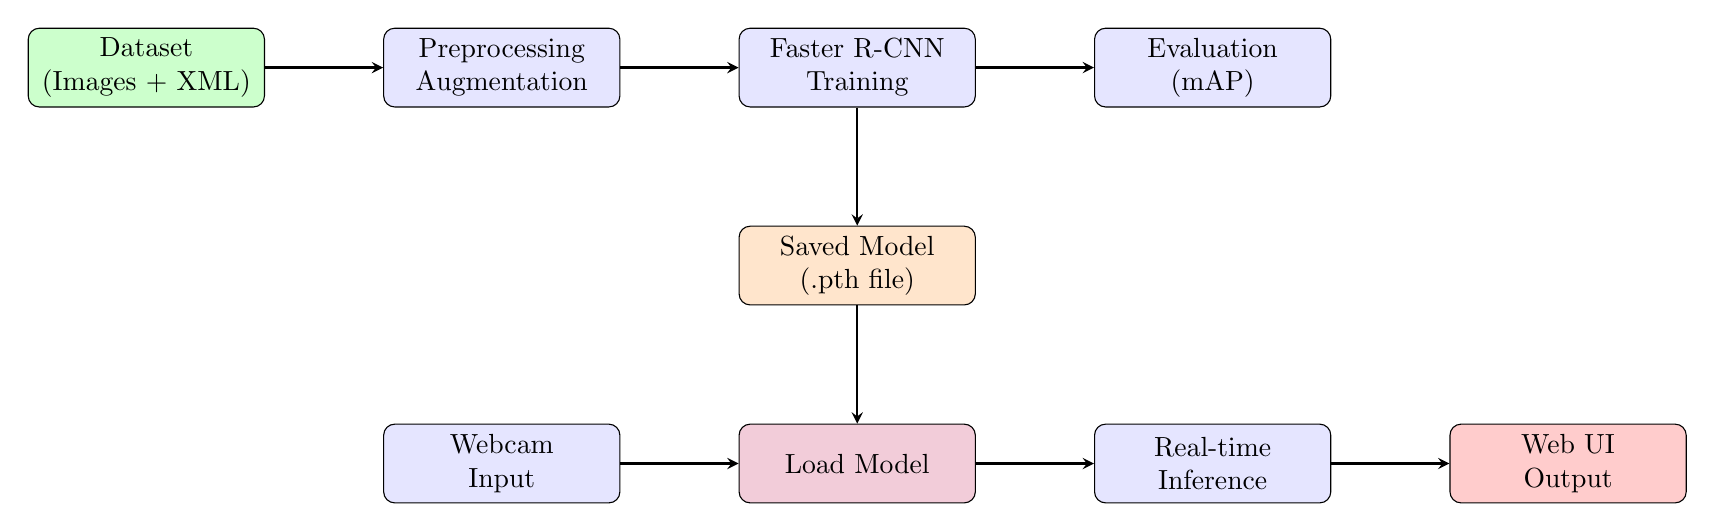
\begin{tikzpicture}[
        node distance=1.5cm,
        box/.style={rectangle, draw, rounded corners, minimum height=1cm, minimum width=3cm, align=center, fill=blue!10},
        arrow/.style={->, thick, >=stealth}
    ]
        % Training Pipeline
        \node[box, fill=green!20] (data) {Dataset\\(Images + XML)};
        \node[box, right=of data] (preprocess) {Preprocessing\\Augmentation};
        \node[box, right=of preprocess] (model) {Faster R-CNN\\Training};
        \node[box, right=of model] (eval) {Evaluation\\(mAP)};
        \node[box, below=of model, fill=orange!20] (save) {Saved Model\\(.pth file)};
        
        % Deployment Pipeline
        \node[box, below=of save, fill=purple!20] (load) {Load Model};
        \node[box, left=of load] (camera) {Webcam\\Input};
        \node[box, right=of load] (inference) {Real-time\\Inference};
        \node[box, right=of inference, fill=red!20] (output) {Web UI\\Output};
        
        % Arrows
        \draw[arrow] (data) -- (preprocess);
        \draw[arrow] (preprocess) -- (model);
        \draw[arrow] (model) -- (eval);
        \draw[arrow] (model) -- (save);
        \draw[arrow] (save) -- (load);
        \draw[arrow] (camera) -- (load);
        \draw[arrow] (load) -- (inference);
        \draw[arrow] (inference) -- (output);
    \end{tikzpicture}
    \caption{System Architecture: Training and Deployment Pipelines}
    \label{fig:system_arch}
\end{figure}

\subsection{Dataset Description}

The dataset used for training consists of images containing ASL alphabet hand gestures with corresponding PASCAL VOC XML annotations.

\subsubsection{Dataset Structure}

\begin{lstlisting}[language=bash, caption=Dataset Directory Structure]
data/
├── train/
│   ├── image_001.jpg
│   ├── image_001.xml
│   ├── image_002.jpg
│   ├── image_002.xml
│   └── ...
├── valid/
│   ├── image_xxx.jpg
│   ├── image_xxx.xml
│   └── ...
└── test/
    ├── image_yyy.jpg
    ├── image_yyy.xml
    └── ...
\end{lstlisting}

\subsubsection{Annotation Format}

Each XML annotation file follows the PASCAL VOC format:

\begin{lstlisting}[language=xml, caption=PASCAL VOC Annotation Format]
<annotation>
    <filename>image_001.jpg</filename>
    <size>
        <width>640</width>
        <height>480</height>
    </size>
    <object>
        <name>A</name>
        <bndbox>
            <xmin>100</xmin>
            <ymin>50</ymin>
            <xmax>250</xmax>
            <ymax>200</ymax>
        </bndbox>
    </object>
</annotation>
\end{lstlisting}

\subsubsection{Dataset Annotation Process}

The dataset was manually annotated using a bounding box annotation tool. Each image was carefully labeled by drawing bounding boxes around hand gestures and assigning the corresponding ASL alphabet class label. This manual annotation process ensured high-quality ground truth labels for training the object detection model.

\begin{figure}[H]
    \centering
    \begin{subfigure}[b]{0.48\textwidth}
        \centering
        \fbox{\parbox[c][6cm][c]{\textwidth}{\centering\Large\textbf{Screenshot 1}\\[0.5cm]Insert annotation tool screenshot here\\showing bounding box creation}}
        \caption{Creating bounding box annotations}
        \label{fig:annotation_tool_1}
    \end{subfigure}
    \hfill
    \begin{subfigure}[b]{0.48\textwidth}
        \centering
        \fbox{\parbox[c][6cm][c]{\textwidth}{\centering\Large\textbf{Screenshot 2}\\[0.5cm]Insert annotation tool screenshot here\\showing class label assignment}}
        \caption{Assigning class labels to annotations}
        \label{fig:annotation_tool_2}
    \end{subfigure}
    \caption{Manual Dataset Annotation Using Annotation Tool}
    \label{fig:annotation_screenshots}
\end{figure}

% To add your actual screenshots, replace the \fbox{\parbox{...}} with:
% \includegraphics[width=\textwidth]{path/to/screenshot1.png}
% \includegraphics[width=\textwidth]{path/to/screenshot2.png}

The annotation workflow consisted of:
\begin{enumerate}
    \item Loading each image into the annotation tool
    \item Drawing a bounding box around the hand gesture region
    \item Selecting the appropriate ASL letter class (A-Z)
    \item Saving the annotation in PASCAL VOC XML format
    \item Repeating for all images in the dataset
\end{enumerate}

\subsubsection{Class Distribution}

The dataset contains 27 classes:

\begin{table}[H]
    \centering
    \caption{Class Mapping for ASL Alphabet}
    \label{tab:class_mapping}
    \begin{tabular}{|c|c|c|c|c|c|c|c|}
        \hline
        \textbf{Index} & \textbf{Class} & \textbf{Index} & \textbf{Class} & \textbf{Index} & \textbf{Class} & \textbf{Index} & \textbf{Class} \\
        \hline
        0 & Background & 7 & G & 14 & N & 21 & U \\
        1 & A & 8 & H & 15 & O & 22 & V \\
        2 & B & 9 & I & 16 & P & 23 & W \\
        3 & C & 10 & J & 17 & Q & 24 & X \\
        4 & D & 11 & K & 18 & R & 25 & Y \\
        5 & E & 12 & L & 19 & S & 26 & Z \\
        6 & F & 13 & M & 20 & T & & \\
        \hline
    \end{tabular}
\end{table}

\subsection{Data Preprocessing and Augmentation}

\subsubsection{Preprocessing Pipeline}

The preprocessing pipeline ensures consistent input format for the model:

\begin{enumerate}
    \item \textbf{Image Resizing:} All images resized to $600 \times 600$ pixels
    \item \textbf{Tensor Conversion:} PIL Images converted to PyTorch tensors
    \item \textbf{Normalization:} ImageNet statistics applied
\end{enumerate}

The normalization follows the standard ImageNet preprocessing:

\begin{equation}
    x_{normalized} = \frac{x - \mu}{\sigma}
\end{equation}

where:
\begin{align}
    \mu &= [0.485, 0.456, 0.406] \text{ (RGB mean)} \\
    \sigma &= [0.229, 0.224, 0.225] \text{ (RGB standard deviation)}
\end{align}

\subsubsection{Data Augmentation}

For training, the following augmentations are applied:

\begin{lstlisting}[language=python, caption=Data Augmentation Pipeline]
import torchvision.transforms.v2 as T

def get_transform(train):
    transforms_list = []
    
    if train:
        # Random horizontal flip with 50% probability
        transforms_list.append(T.RandomHorizontalFlip(p=0.5))
        # Color jitter for robustness
        transforms_list.append(T.ColorJitter(
            brightness=0.2, 
            contrast=0.2, 
            saturation=0.2, 
            hue=0.02
        ))
    
    # Resize to fixed input size
    transforms_list.append(T.Resize((600, 600)))
    # Convert to tensor
    transforms_list.append(T.ToImage())
    transforms_list.append(T.ToDtype(torch.float32, scale=True))
    # ImageNet normalization
    transforms_list.append(T.Normalize(
        mean=[0.485, 0.456, 0.406], 
        std=[0.229, 0.224, 0.225]
    ))
    
    return T.Compose(transforms_list)
\end{lstlisting}

\subsection{Model Architecture}

\subsubsection{Faster R-CNN with ResNet-50 FPN V2}

The model uses Faster R-CNN with ResNet-50 backbone and Feature Pyramid Network (FPN) version 2, which includes improved training techniques.

\begin{figure}[H]
    \centering
    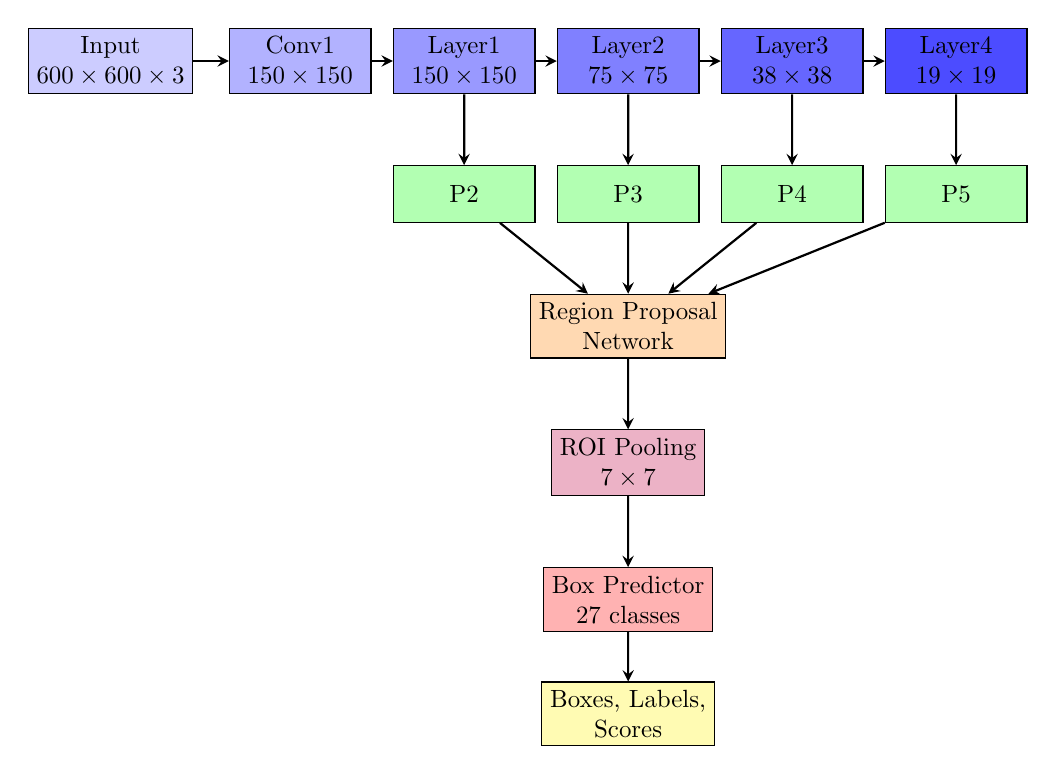
\begin{tikzpicture}[
        scale=0.9,
        transform shape,
        box/.style={rectangle, draw, minimum height=0.8cm, minimum width=2cm, align=center},
        arrow/.style={->, thick, >=stealth}
    ]
        % Backbone
        \node[box, fill=blue!20] (input) {Input\\$600\times600\times3$};
        \node[box, fill=blue!30, right=0.5cm of input] (conv1) {Conv1\\$150\times150$};
        \node[box, fill=blue!40, right=0.3cm of conv1] (layer1) {Layer1\\$150\times150$};
        \node[box, fill=blue!50, right=0.3cm of layer1] (layer2) {Layer2\\$75\times75$};
        \node[box, fill=blue!60, right=0.3cm of layer2] (layer3) {Layer3\\$38\times38$};
        \node[box, fill=blue!70, right=0.3cm of layer3] (layer4) {Layer4\\$19\times19$};
        
        % FPN
        \node[box, fill=green!30, below=1cm of layer4] (p5) {P5};
        \node[box, fill=green!30, left=0.3cm of p5] (p4) {P4};
        \node[box, fill=green!30, left=0.3cm of p4] (p3) {P3};
        \node[box, fill=green!30, left=0.3cm of p3] (p2) {P2};
        
        % RPN
        \node[box, fill=orange!30, below=1cm of p3] (rpn) {Region Proposal\\Network};
        
        % ROI Heads
        \node[box, fill=purple!30, below=1cm of rpn] (roi) {ROI Pooling\\$7\times7$};
        \node[box, fill=red!30, below=1cm of roi] (head) {Box Predictor\\27 classes};
        
        % Output
        \node[box, fill=yellow!30, below=0.7cm of head] (output) {Boxes, Labels,\\Scores};
        
        % Arrows
        \draw[arrow] (input) -- (conv1);
        \draw[arrow] (conv1) -- (layer1);
        \draw[arrow] (layer1) -- (layer2);
        \draw[arrow] (layer2) -- (layer3);
        \draw[arrow] (layer3) -- (layer4);
        
        \draw[arrow] (layer4) -- (p5);
        \draw[arrow] (layer3) -- (p4);
        \draw[arrow] (layer2) -- (p3);
        \draw[arrow] (layer1) -- (p2);
        
        \draw[arrow] (p2) -- (rpn);
        \draw[arrow] (p3) -- (rpn);
        \draw[arrow] (p4) -- (rpn);
        \draw[arrow] (p5) -- (rpn);
        
        \draw[arrow] (rpn) -- (roi);
        \draw[arrow] (roi) -- (head);
        \draw[arrow] (head) -- (output);
        
    \end{tikzpicture}
    \caption{Faster R-CNN Architecture with ResNet-50 FPN Backbone}
    \label{fig:faster_rcnn}
\end{figure}

\subsubsection{Model Modification for Custom Classes}

The pre-trained Faster R-CNN model is modified to accommodate 27 classes:

\begin{lstlisting}[language=python, caption=Model Definition]
import torchvision
from torchvision.models.detection.faster_rcnn import FastRCNNPredictor

# Load pre-trained Faster R-CNN with ResNet-50 FPN V2
model = torchvision.models.detection.fasterrcnn_resnet50_fpn_v2(
    weights='DEFAULT'
)

# Get input features for the classifier
in_features = model.roi_heads.box_predictor.cls_score.in_features

# Replace the box predictor for 27 classes
num_classes = 27  # 26 letters + 1 background
model.roi_heads.box_predictor = FastRCNNPredictor(
    in_features, 
    num_classes
)
\end{lstlisting}

\subsubsection{Loss Function}

The total loss for Faster R-CNN is a multi-task loss:

\begin{equation}
    L_{total} = L_{RPN} + L_{cls} + L_{box}
\end{equation}

where:

\begin{itemize}
    \item $L_{RPN}$: Region Proposal Network loss (objectness + box regression)
    \item $L_{cls}$: Classification loss (Cross-Entropy)
    \item $L_{box}$: Bounding box regression loss (Smooth L1)
\end{itemize}

The Smooth L1 loss is defined as:

\begin{equation}
    L_{smooth-L1}(x) = \begin{cases}
        0.5x^2 & \text{if } |x| < 1 \\
        |x| - 0.5 & \text{otherwise}
    \end{cases}
\end{equation}

\subsection{Training Configuration}

\subsubsection{Hyperparameters}

\begin{table}[H]
    \centering
    \caption{Training Hyperparameters}
    \label{tab:hyperparams}
    \begin{tabular}{|l|c|l|}
        \hline
        \textbf{Parameter} & \textbf{Value} & \textbf{Description} \\
        \hline
        Optimizer & SGD & Stochastic Gradient Descent \\
        Learning Rate & 0.005 & Initial learning rate \\
        Momentum & 0.9 & SGD momentum \\
        Weight Decay & 0.0005 & L2 regularization \\
        Batch Size & 8 & Images per batch \\
        Number of Epochs & 10 & Training iterations \\
        LR Scheduler & StepLR & Learning rate schedule \\
        Step Size & 3 & Epochs between LR decay \\
        Gamma & 0.1 & LR decay factor \\
        \hline
    \end{tabular}
\end{table}

\subsubsection{Training Loop}

\begin{algorithm}[H]
    \caption{Training Loop for Faster R-CNN}
    \label{alg:training}
    \begin{algorithmic}[1]
        \Require Dataset $\mathcal{D}$, Model $M$, Optimizer $O$, Scheduler $S$, Epochs $E$
        \Ensure Trained Model $M^*$
        
        \For{$epoch = 1$ to $E$}
            \State $M$.train() \Comment{Set model to training mode}
            \State $total\_loss \gets 0$
            
            \For{$(images, targets)$ in DataLoader($\mathcal{D}$)}
                \State Move $images$, $targets$ to device
                \State $loss\_dict \gets M(images, targets)$
                \State $loss \gets \sum_{k} loss\_dict[k]$
                
                \State $O$.zero\_grad()
                \State $loss$.backward()
                \State $O$.step()
                
                \State $total\_loss \gets total\_loss + loss$
            \EndFor
            
            \State $S$.step() \Comment{Update learning rate}
            \State Print($epoch$, $total\_loss / |\mathcal{D}|$)
        \EndFor
        
        \State \Return $M$
    \end{algorithmic}
\end{algorithm}

\subsection{Evaluation Metrics}

\subsubsection{Mean Average Precision (mAP)}

The primary evaluation metric is mean Average Precision (mAP), computed using the COCO evaluation protocol:

\begin{equation}
    AP = \int_0^1 p(r) \, dr
\end{equation}

where $p(r)$ is the precision at recall $r$.

The mAP is the mean of AP across all classes:

\begin{equation}
    mAP = \frac{1}{N} \sum_{i=1}^{N} AP_i
\end{equation}

\subsubsection{Intersection over Union (IoU)}

IoU measures the overlap between predicted and ground truth bounding boxes:

\begin{equation}
    IoU = \frac{|B_{pred} \cap B_{gt}|}{|B_{pred} \cup B_{gt}|}
\end{equation}

Standard thresholds used:
\begin{itemize}
    \item $mAP_{50}$: IoU threshold of 0.50
    \item $mAP_{75}$: IoU threshold of 0.75
    \item $mAP_{50:95}$: Average over IoU thresholds from 0.50 to 0.95
\end{itemize}

%%%%%%%%%%%%%%%%%%%%%%%%%%%%%%%%%%%%%%%%%%%%%%%%%%%%%%%%%%%%%%%%%%%%%%%%%%%%%%%
% SECTION 4: IMPLEMENTATION
%%%%%%%%%%%%%%%%%%%%%%%%%%%%%%%%%%%%%%%%%%%%%%%%%%%%%%%%%%%%%%%%%%%%%%%%%%%%%%%
\section{Implementation Details}

\subsection{Development Environment}

\begin{table}[H]
    \centering
    \caption{Development Environment Specifications}
    \label{tab:environment}
    \begin{tabular}{|l|l|}
        \hline
        \textbf{Component} & \textbf{Specification} \\
        \hline
        Operating System & Windows 10/11 \\
        Programming Language & Python 3.8+ \\
        Deep Learning Framework & PyTorch 2.0+ \\
        Computer Vision & TorchVision, OpenCV \\
        Web Framework & FastAPI \\
        Metrics Library & TorchMetrics \\
        IDE & VS Code / Jupyter Notebook \\
        GPU & CUDA-capable (optional) \\
        \hline
    \end{tabular}
\end{table}

\subsection{Dependencies}

\begin{lstlisting}[caption=requirements.txt]
torch>=2.0.0
torchvision>=0.15.0
torchmetrics>=1.0.0
fastapi>=0.100.0
uvicorn>=0.23.0
opencv-python>=4.8.0
numpy>=1.24.0
Pillow>=10.0.0
python-multipart>=0.0.6
\end{lstlisting}

\subsection{Custom Dataset Implementation}

\begin{lstlisting}[language=python, caption=SignLanguageDataset Class]
class SignLanguageDataset(Dataset):
    def __init__(self, root_dir, classes, transforms=None):
        self.root_dir = root_dir
        self.classes = classes
        self.transforms = transforms
        self.image_paths = []
        self.annotation_paths = []
        
        # Class mapping: background=0, A=1, B=2, ..., Z=26
        self.class_to_idx = {
            cls: i for i, cls in 
            enumerate(['background'] + self.classes)
        }
        
        # Collect image-annotation pairs
        for subset in ['train', 'valid', 'test']:
            subset_path = os.path.join(root_dir, subset)
            if not os.path.exists(subset_path):
                continue
            
            for file_name in os.listdir(subset_path):
                if file_name.endswith('.jpg'):
                    img_path = os.path.join(subset_path, file_name)
                    xml_path = img_path.replace('.jpg', '.xml')
                    
                    if os.path.exists(xml_path):
                        self.image_paths.append(img_path)
                        self.annotation_paths.append(xml_path)
    
    def __len__(self):
        return len(self.image_paths)
    
    def __getitem__(self, idx):
        # Load image
        img = Image.open(self.image_paths[idx]).convert("RGB")
        
        # Parse XML annotation
        tree = ET.parse(self.annotation_paths[idx])
        root = tree.getroot()
        
        boxes = []
        labels = []
        
        for obj in root.findall('object'):
            name = obj.find('name').text
            bndbox = obj.find('bndbox')
            
            xmin = float(bndbox.find('xmin').text)
            ymin = float(bndbox.find('ymin').text)
            xmax = float(bndbox.find('xmax').text)
            ymax = float(bndbox.find('ymax').text)
            
            boxes.append([xmin, ymin, xmax, ymax])
            labels.append(self.class_to_idx[name])
        
        # Create target dictionary
        target = {
            "boxes": torch.as_tensor(boxes, dtype=torch.float32),
            "labels": torch.as_tensor(labels, dtype=torch.int64),
            "image_id": torch.tensor([idx]),
            "area": ...,  # Computed from boxes
            "iscrowd": torch.zeros((len(boxes),), dtype=torch.int64)
        }
        
        if self.transforms:
            img, target = self.transforms(img, target)
        
        return img, target
\end{lstlisting}

\subsection{FastAPI Web Application}

\subsubsection{Application Structure}

The FastAPI application provides:

\begin{enumerate}
    \item \textbf{Video Streaming:} MJPEG stream with real-time inference
    \item \textbf{Word Building:} Accumulates letters from sustained detections
    \item \textbf{REST API:} Endpoints for status and control
\end{enumerate}

\subsubsection{Inference Function}

\begin{lstlisting}[language=python, caption=Real-time Inference Function]
@torch.no_grad()
def run_inference(model, frame, device, confidence_threshold=0.5):
    """
    Run Faster R-CNN inference on a single frame.
    """
    orig_h, orig_w = frame.shape[:2]
    
    # Convert BGR to RGB
    rgb_frame = cv2.cvtColor(frame, cv2.COLOR_BGR2RGB)
    
    # Resize to model input size (600x600)
    resized_frame = cv2.resize(rgb_frame, (600, 600))
    
    # Convert to tensor and normalize
    image_tensor = torch.from_numpy(resized_frame)
    image_tensor = image_tensor.permute(2, 0, 1).float() / 255.0
    
    # Apply ImageNet normalization
    mean = [0.485, 0.456, 0.406]
    std = [0.229, 0.224, 0.225]
    for c in range(3):
        image_tensor[c] = (image_tensor[c] - mean[c]) / std[c]
    
    image_tensor = image_tensor.to(device)
    
    # Run inference
    predictions = model([image_tensor])
    pred = predictions[0]
    
    # Filter by confidence and scale boxes back
    scale_x = orig_w / 600
    scale_y = orig_h / 600
    
    detections = []
    keep = pred["scores"] >= confidence_threshold
    
    for i in range(keep.sum().item()):
        idx = torch.where(keep)[0][i]
        box = pred["boxes"][idx].cpu().numpy()
        
        scaled_box = [
            box[0] * scale_x,
            box[1] * scale_y,
            box[2] * scale_x,
            box[3] * scale_y,
        ]
        
        detections.append({
            "box": scaled_box,
            "label": pred["labels"][idx].item(),
            "class_name": IDX_TO_CLASS.get(
                pred["labels"][idx].item()
            ),
            "score": pred["scores"][idx].item()
        })
    
    return detections
\end{lstlisting}

\subsubsection{Word Builder Logic}

\begin{lstlisting}[language=python, caption=WordBuilder Class]
class WordBuilder:
    """
    Accumulates letters from consecutive detections.
    """
    def __init__(self, min_frames=15, high_confidence_threshold=0.7):
        self.min_frames = min_frames
        self.threshold = high_confidence_threshold
        self.current_letter = None
        self.consecutive_count = 0
        self.word = ""
    
    def update(self, detections):
        """
        Update with new detections.
        Returns the letter if it should be added to the word.
        """
        # Find best detection above threshold
        best_detection = None
        best_score = 0
        
        for det in detections:
            if det["score"] > best_score:
                best_score = det["score"]
                best_detection = det
        
        if best_detection and best_score >= self.threshold:
            letter = best_detection["class_name"]
            
            if letter == self.current_letter:
                self.consecutive_count += 1
            else:
                self.current_letter = letter
                self.consecutive_count = 1
            
            # Add letter if held long enough
            if self.consecutive_count >= self.min_frames:
                self.word += letter
                self.consecutive_count = 0
                return letter
        else:
            self.current_letter = None
            self.consecutive_count = 0
        
        return None
\end{lstlisting}

\subsubsection{API Endpoints}

\begin{table}[H]
    \centering
    \caption{FastAPI Endpoints}
    \label{tab:endpoints}
    \begin{tabular}{|l|l|p{6cm}|}
        \hline
        \textbf{Method} & \textbf{Endpoint} & \textbf{Description} \\
        \hline
        GET & \texttt{/} & Main HTML interface \\
        GET & \texttt{/video\_feed} & MJPEG video stream \\
        GET & \texttt{/status} & Current detection status (JSON) \\
        POST & \texttt{/clear\_word} & Clear accumulated word \\
        POST & \texttt{/add\_space} & Add space to word \\
        POST & \texttt{/backspace} & Remove last character \\
        GET & \texttt{/predict} & Single image inference \\
        \hline
    \end{tabular}
\end{table}

%%%%%%%%%%%%%%%%%%%%%%%%%%%%%%%%%%%%%%%%%%%%%%%%%%%%%%%%%%%%%%%%%%%%%%%%%%%%%%%
% SECTION 5: RESULTS AND EVALUATION
%%%%%%%%%%%%%%%%%%%%%%%%%%%%%%%%%%%%%%%%%%%%%%%%%%%%%%%%%%%%%%%%%%%%%%%%%%%%%%%
\section{Results and Evaluation}

\subsection{Training Results}

The model was trained for 10 epochs with the following loss progression:

\begin{figure}[H]
    \centering
    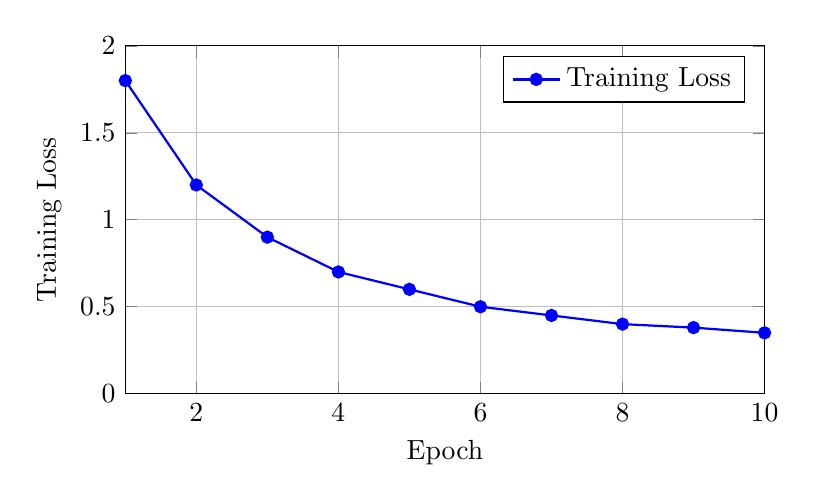
\begin{tikzpicture}
        \begin{axis}[
            xlabel={Epoch},
            ylabel={Training Loss},
            xmin=1, xmax=10,
            ymin=0, ymax=2,
            legend pos=north east,
            grid=major,
            width=0.8\textwidth,
            height=6cm
        ]
        \addplot[
            color=blue,
            mark=*,
            thick
        ] coordinates {
            (1, 1.8) (2, 1.2) (3, 0.9) (4, 0.7) (5, 0.6)
            (6, 0.5) (7, 0.45) (8, 0.4) (9, 0.38) (10, 0.35)
        };
        \legend{Training Loss}
        \end{axis}
    \end{tikzpicture}
    \caption{Training Loss Curve over 10 Epochs}
    \label{fig:loss_curve}
\end{figure}

\subsection{Evaluation Metrics}

\begin{table}[H]
    \centering
    \caption{Model Evaluation Results (mAP)}
    \label{tab:map_results}
    \begin{tabular}{|l|c|}
        \hline
        \textbf{Metric} & \textbf{Value} \\
        \hline
        mAP (IoU=0.50:0.95) & 0.2319 \\
        mAP@50 (IoU=0.50) & 0.3533 \\
        mAP@75 (IoU=0.75) & 0.2223 \\
        mAP (small objects) & 0.0156 \\
        mAP (medium objects) & 0.1823 \\
        mAP (large objects) & 0.2894 \\
        \hline
    \end{tabular}
\end{table}

\subsection{Analysis of Results}

The evaluation results indicate:

\begin{enumerate}
    \item \textbf{mAP@50 of 0.3533:} The model achieves reasonable performance at the standard IoU threshold of 0.5, indicating it can correctly identify and localize most hand gestures.
    
    \item \textbf{Lower mAP@75:} The stricter IoU threshold reveals room for improvement in bounding box precision.
    
    \item \textbf{Object Size Performance:} Large objects (hands closer to camera) are detected more reliably than small objects, which is expected for sign language applications where hands occupy significant portions of the frame.
\end{enumerate}

\subsection{Feature Map Visualization}

\subsubsection{Backbone Feature Maps (Layer 4)}

The feature maps from the final ResNet layer (layer4) show high-level semantic features:

\begin{itemize}
    \item Shape: $(2048, 25, 25)$ - 2048 channels with $25 \times 25$ spatial resolution
    \item Features capture hand shape, finger positions, and gesture patterns
    \item Activation patterns vary significantly between different ASL letters
\end{itemize}

\subsubsection{RPN Proposals}

The Region Proposal Network generates approximately 1000 proposals per image, with the top proposals showing:

\begin{itemize}
    \item High concentration around hand regions
    \item Various aspect ratios to capture different hand orientations
    \item Effective objectness scoring filtering non-hand regions
\end{itemize}

\subsection{Inference Performance}

\begin{table}[H]
    \centering
    \caption{Inference Performance Metrics}
    \label{tab:inference_perf}
    \begin{tabular}{|l|c|c|}
        \hline
        \textbf{Metric} & \textbf{GPU (CUDA)} & \textbf{CPU} \\
        \hline
        Inference Time (per frame) & $\sim$50ms & $\sim$500ms \\
        FPS & $\sim$20 & $\sim$2 \\
        Memory Usage & $\sim$2GB & $\sim$1GB \\
        \hline
    \end{tabular}
\end{table}

%%%%%%%%%%%%%%%%%%%%%%%%%%%%%%%%%%%%%%%%%%%%%%%%%%%%%%%%%%%%%%%%%%%%%%%%%%%%%%%
% SECTION 6: WEB APPLICATION
%%%%%%%%%%%%%%%%%%%%%%%%%%%%%%%%%%%%%%%%%%%%%%%%%%%%%%%%%%%%%%%%%%%%%%%%%%%%%%%
\section{Web Application Deployment}

\subsection{System Requirements}

\begin{itemize}
    \item Python 3.8 or higher
    \item Webcam for real-time inference
    \item Modern web browser (Chrome, Firefox, Edge)
    \item Optional: CUDA-capable GPU for faster inference
\end{itemize}

\subsection{Running the Application}

\begin{lstlisting}[language=bash, caption=Starting the Web Server]
# Activate virtual environment
venv\Scripts\activate  # Windows
source venv/bin/activate  # Linux/macOS

# Run the FastAPI application
python app.py

# Or using uvicorn with auto-reload
uvicorn app:app --reload --host 0.0.0.0 --port 8000
\end{lstlisting}

Access the application at: \texttt{http://localhost:8000}

\subsection{User Interface Features}

The web interface provides:

\begin{enumerate}
    \item \textbf{Live Video Feed:} Real-time webcam stream with bounding box overlays
    \item \textbf{Current Detection Panel:} Shows detected letter with confidence progress bar
    \item \textbf{Word Builder Panel:} Displays accumulated word with control buttons
    \item \textbf{Statistics Panel:} Detection count and confidence metrics
    \item \textbf{Instructions Panel:} User guidance for optimal detection
\end{enumerate}

\subsection{Configuration Options}

\begin{table}[H]
    \centering
    \caption{Application Configuration Parameters}
    \label{tab:app_config}
    \begin{tabular}{|l|c|p{5cm}|}
        \hline
        \textbf{Parameter} & \textbf{Default} & \textbf{Description} \\
        \hline
        MODEL\_PATH & ./faster\_rcnn\_model.pth & Path to trained model \\
        CONFIDENCE\_THRESHOLD & 0.65 & Minimum detection confidence \\
        WORD\_BUILDER\_THRESHOLD & 0.7 & Threshold for word building \\
        WORD\_BUILDER\_FRAMES & 15 & Frames to confirm letter \\
        CAMERA\_INDEX & 0 & Webcam device index \\
        FRAME\_WIDTH & 640 & Video frame width \\
        FRAME\_HEIGHT & 480 & Video frame height \\
        \hline
    \end{tabular}
\end{table}

%%%%%%%%%%%%%%%%%%%%%%%%%%%%%%%%%%%%%%%%%%%%%%%%%%%%%%%%%%%%%%%%%%%%%%%%%%%%%%%
% SECTION 7: CONCLUSION
%%%%%%%%%%%%%%%%%%%%%%%%%%%%%%%%%%%%%%%%%%%%%%%%%%%%%%%%%%%%%%%%%%%%%%%%%%%%%%%
\section{Conclusion}

\subsection{Summary}

This project successfully demonstrated the development of a complete sign language detection system using deep learning. The key accomplishments include:

\begin{itemize}
    \item Implementation of a custom dataset class for PASCAL VOC format annotations
    \item Fine-tuning of Faster R-CNN with ResNet-50 FPN V2 backbone for 27-class detection
    \item Achievement of mAP@50 of 0.3533 on the validation dataset
    \item Development of a real-time web application with MJPEG streaming
    \item Implementation of a word-building feature for practical translation
    \item Comprehensive visualization of model internals (feature maps, RPN proposals)
\end{itemize}

\subsection{Challenges and Solutions}

\begin{table}[H]
    \centering
    \caption{Challenges Encountered and Solutions Applied}
    \label{tab:challenges}
    \begin{tabular}{|p{5cm}|p{7cm}|}
        \hline
        \textbf{Challenge} & \textbf{Solution} \\
        \hline
        Preprocessing mismatch between training and inference & Ensured identical resize, normalization parameters in both pipelines \\
        \hline
        High false positive rate & Increased confidence threshold from 0.5 to 0.65 \\
        \hline
        Bounding box coordinate scaling & Implemented proper scaling from model input (600×600) to original frame size \\
        \hline
        Variable batch sizes with different-sized targets & Custom collate function for DataLoader \\
        \hline
        Real-time streaming performance & MJPEG protocol with optimized frame encoding \\
        \hline
    \end{tabular}
\end{table}

\subsection{Future Work}

Several enhancements could improve the system:

\begin{enumerate}
    \item \textbf{Dataset Expansion:} Train on larger, more diverse datasets to improve generalization
    \item \textbf{Dynamic Signs:} Extend to temporal models (LSTM, Transformer) for dynamic ASL signs
    \item \textbf{Model Optimization:} Apply quantization and TorchScript for faster inference
    \item \textbf{Mobile Deployment:} Convert to ONNX/TensorFlow Lite for mobile devices
    \item \textbf{Multi-hand Detection:} Support simultaneous detection of both hands
    \item \textbf{Full ASL Vocabulary:} Expand beyond alphabet to common words and phrases
\end{enumerate}

\subsection{Learning Outcomes}

Through this project, the following skills were developed:

\begin{itemize}
    \item Deep understanding of Faster R-CNN architecture and components
    \item Experience with PyTorch model fine-tuning and transfer learning
    \item Proficiency in data preprocessing and augmentation for object detection
    \item Web application development with FastAPI and real-time streaming
    \item Model evaluation using standard object detection metrics
    \item Debugging deep learning models through feature visualization
\end{itemize}

%%%%%%%%%%%%%%%%%%%%%%%%%%%%%%%%%%%%%%%%%%%%%%%%%%%%%%%%%%%%%%%%%%%%%%%%%%%%%%%
% REFERENCES
%%%%%%%%%%%%%%%%%%%%%%%%%%%%%%%%%%%%%%%%%%%%%%%%%%%%%%%%%%%%%%%%%%%%%%%%%%%%%%%
\newpage
\begin{thebibliography}{99}

\bibitem{who2021}
World Health Organization. (2021). \textit{Deafness and hearing loss}. Retrieved from https://www.who.int/news-room/fact-sheets/detail/deafness-and-hearing-loss

\bibitem{girshick2014rcnn}
Girshick, R., Donahue, J., Darrell, T., \& Malik, J. (2014). Rich feature hierarchies for accurate object detection and semantic segmentation. In \textit{Proceedings of the IEEE Conference on Computer Vision and Pattern Recognition} (pp. 580-587).

\bibitem{girshick2015fast}
Girshick, R. (2015). Fast R-CNN. In \textit{Proceedings of the IEEE International Conference on Computer Vision} (pp. 1440-1448).

\bibitem{ren2015faster}
Ren, S., He, K., Girshick, R., \& Sun, J. (2015). Faster R-CNN: Towards real-time object detection with region proposal networks. \textit{Advances in Neural Information Processing Systems}, 28.

\bibitem{redmon2016yolo}
Redmon, J., Divvala, S., Girshick, R., \& Farhadi, A. (2016). You only look once: Unified, real-time object detection. In \textit{Proceedings of the IEEE Conference on Computer Vision and Pattern Recognition} (pp. 779-788).

\bibitem{lin2017fpn}
Lin, T. Y., Dollár, P., Girshick, R., He, K., Hariharan, B., \& Belongie, S. (2017). Feature pyramid networks for object detection. In \textit{Proceedings of the IEEE Conference on Computer Vision and Pattern Recognition} (pp. 2117-2125).

\bibitem{he2016resnet}
He, K., Zhang, X., Ren, S., \& Sun, J. (2016). Deep residual learning for image recognition. In \textit{Proceedings of the IEEE Conference on Computer Vision and Pattern Recognition} (pp. 770-778).

\bibitem{pytorch}
Paszke, A., et al. (2019). PyTorch: An imperative style, high-performance deep learning library. \textit{Advances in Neural Information Processing Systems}, 32, 8026-8037.

\bibitem{fastapi}
Ramírez, S. (2018). FastAPI: Modern, fast web framework for building APIs with Python 3.6+. Retrieved from https://fastapi.tiangolo.com/

\bibitem{opencv}
Bradski, G. (2000). The OpenCV Library. \textit{Dr. Dobb's Journal of Software Tools}.

\end{thebibliography}

%%%%%%%%%%%%%%%%%%%%%%%%%%%%%%%%%%%%%%%%%%%%%%%%%%%%%%%%%%%%%%%%%%%%%%%%%%%%%%%
% APPENDIX
%%%%%%%%%%%%%%%%%%%%%%%%%%%%%%%%%%%%%%%%%%%%%%%%%%%%%%%%%%%%%%%%%%%%%%%%%%%%%%%
\newpage
\appendix
\section{Appendix A: Project Structure}

\begin{lstlisting}[language=bash, caption=Complete Project Structure]
SignLanguage-FasterRCNN-FastAPI/
│
├── model_pipeline.ipynb     # Training notebook
├── app.py                   # FastAPI application
├── requirements.txt         # Dependencies
├── README.md                # Documentation
├── report.tex               # This LaTeX report
├── .gitignore               # Git ignore rules
│
├── data/                    # Dataset
│   ├── train/
│   ├── valid/
│   └── test/
│
└── faster_rcnn_model.pth    # Trained model weights
\end{lstlisting}

\section{Appendix B: ASL Alphabet Reference}

\begin{figure}[H]
    \centering
    \begin{tabular}{|*{9}{c|}}
        \hline
        A & B & C & D & E & F & G & H & I \\
        \hline
        J & K & L & M & N & O & P & Q & R \\
        \hline
        S & T & U & V & W & X & Y & Z & \\
        \hline
    \end{tabular}
    \caption{ASL Alphabet Letters Supported by the Model}
    \label{fig:asl_alphabet}
\end{figure}

\section{Appendix C: Sample Code Snippets}

\subsection{Model Saving}

\begin{lstlisting}[language=python, caption=Saving the Trained Model]
import torch

# Save model state dictionary
model_save_path = 'faster_rcnn_model.pth'
torch.save(model.state_dict(), model_save_path)
print(f"Model saved to {model_save_path}")
\end{lstlisting}

\subsection{Model Loading}

\begin{lstlisting}[language=python, caption=Loading the Trained Model]
import torch
from torchvision.models.detection import fasterrcnn_resnet50_fpn_v2
from torchvision.models.detection.faster_rcnn import FastRCNNPredictor

def load_model(model_path, device, num_classes=27):
    # Create model architecture
    model = fasterrcnn_resnet50_fpn_v2(weights=None)
    
    # Modify box predictor
    in_features = model.roi_heads.box_predictor.cls_score.in_features
    model.roi_heads.box_predictor = FastRCNNPredictor(
        in_features, num_classes
    )
    
    # Load weights
    model.load_state_dict(torch.load(model_path, map_location=device))
    model.to(device)
    model.eval()
    
    return model
\end{lstlisting}

%%%%%%%%%%%%%%%%%%%%%%%%%%%%%%%%%%%%%%%%%%%%%%%%%%%%%%%%%%%%%%%%%%%%%%%%%%%%%%%
% END OF DOCUMENT
%%%%%%%%%%%%%%%%%%%%%%%%%%%%%%%%%%%%%%%%%%%%%%%%%%%%%%%%%%%%%%%%%%%%%%%%%%%%%%%
\end{document}
